
\subsection{2.11. Диаграммы МО для водородных соединений 13-ой – 16-ой групп.} 

\par\bigskip

\begin{figure}[H]
	\centering
	{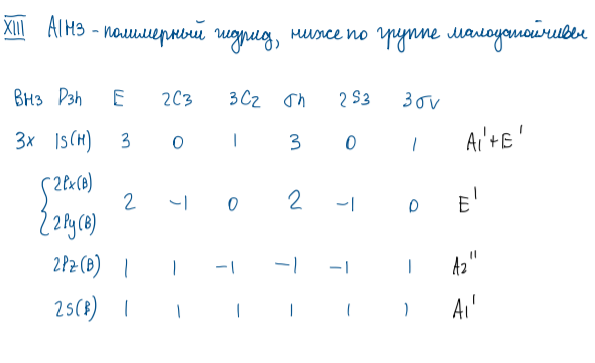
\includegraphics[scale=1]{57.png}}
\end{figure}

\begin{figure}[H]
	\centering
	{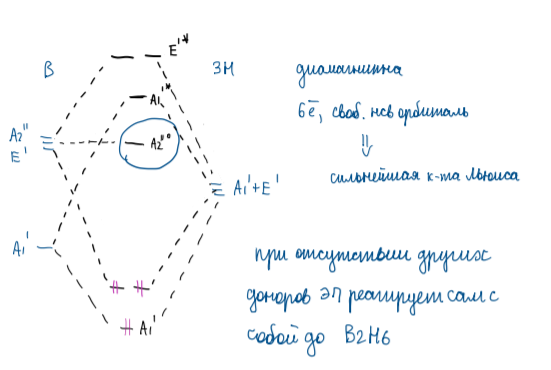
\includegraphics[scale=1]{58.png}}
\end{figure}

\begin{figure}[H]
	\centering
	{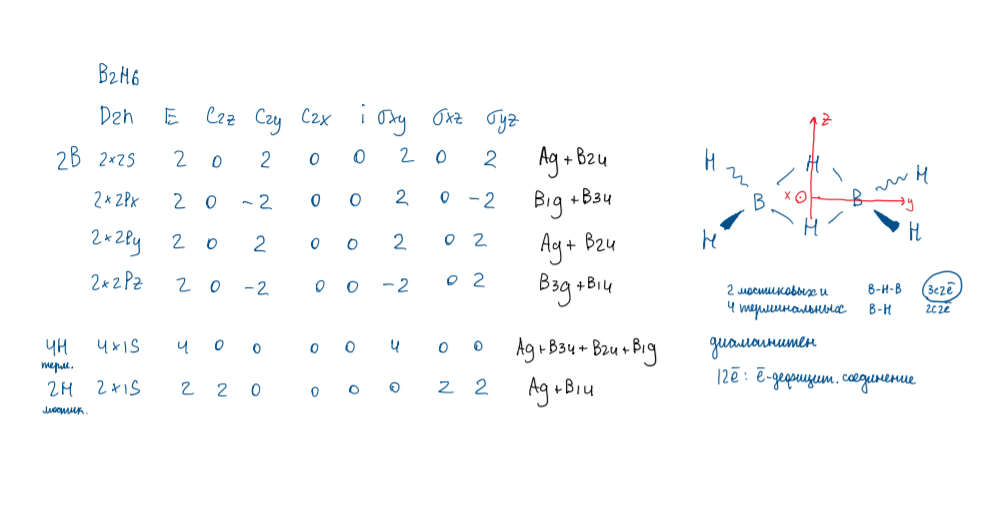
\includegraphics[scale=0.8]{59.png}}
\end{figure}

\begin{figure}[H]
	\centering
	{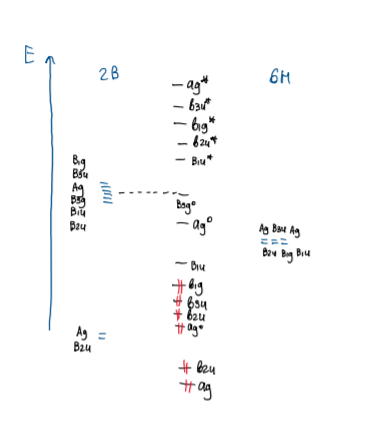
\includegraphics[scale=1]{60.png}}
\end{figure}

\begin{figure}[H]
	\centering
	{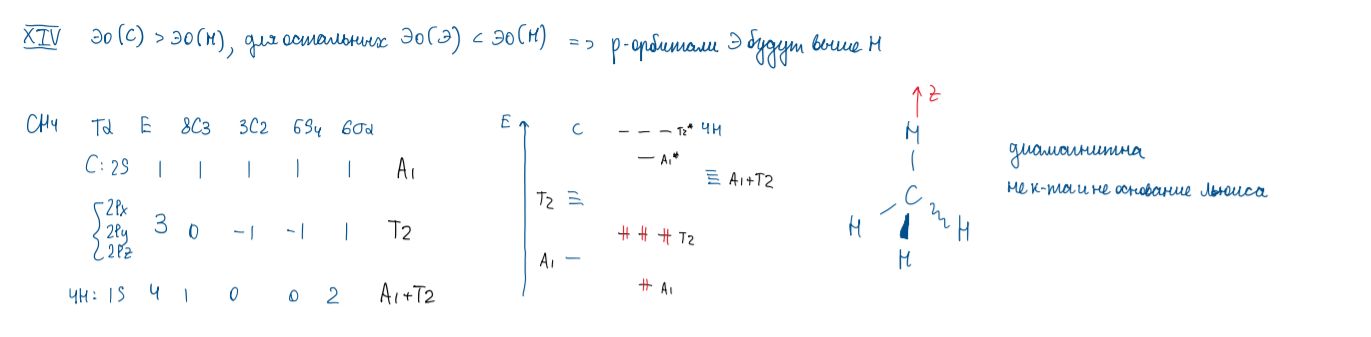
\includegraphics[scale=0.65]{61.png}}
\end{figure}

\begin{figure}[H]
	\centering
	{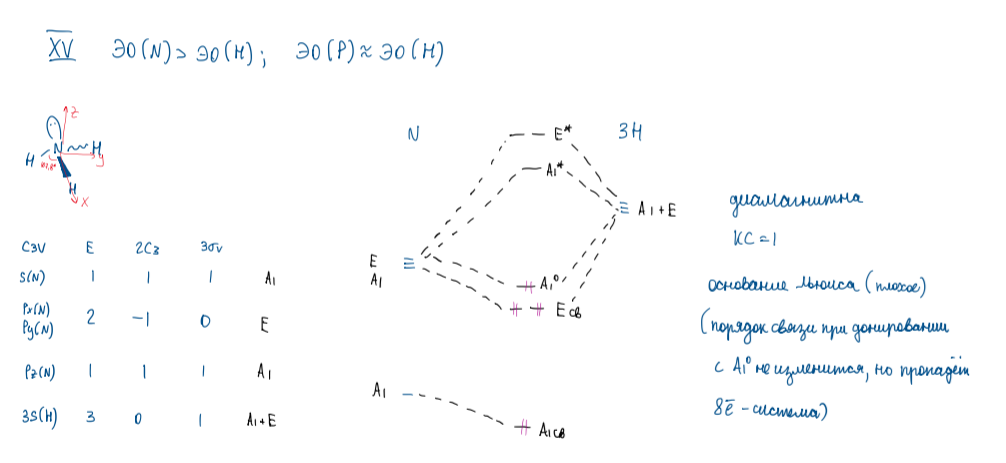
\includegraphics[scale=0.8]{62.png}}
\end{figure}

\begin{figure}[H]
	\centering
	{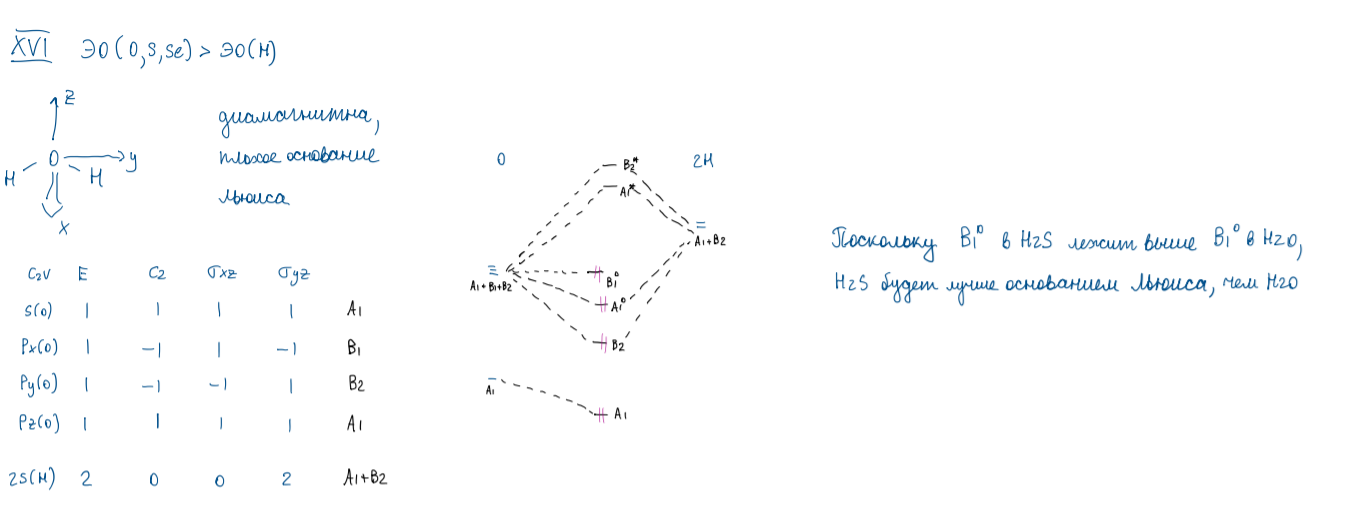
\includegraphics[scale=0.6]{63.png}}
\end{figure}


\par\bigskip
\par\bigskip